\chapter{Clustering}
\label{ch:capitolo2}

This chapter of the report aims at illustrating the clustering analysis performed on the dataset at hand.
The employed clustering techniques are K-means (Centroid-based), DBSCAN (density-based) and hierarchical clustering.
%The analysis conducted using these methods focused on the numeric attributes of the dataset \textbf{CAPIRE SE FARE ANALISI SOLO SU NUMERICHE O INCLUDERE ANCHE BINARIE CON MIXED DISTANCES
%MATRIX}, appropriately log-transformed (as illustrated in the \textit{Variable Transformation} section) and normalized with \textbf{STANDARDSCALER o MINMAX???}.
%To provide a proper visualization of the results, a Principal Component Analysis has been conducted on the preprocessed data. 
%In particular, the optimal number of components that has been found is \textbf{se usiamo solo numeriche dovrebbe essere 4/5} (as in \textbf{AGGIUNGERE FIGURA}).

\section{K-means}\label{sec:centroid_based} %DA AGGIUNGERE SOTTOSEZIONE K-MEANS SE INCLUDIAMO ANCHE BISECTING
The clustering analysis performed with the K-means algorithm focused on the numeric variables of the dataset, excluding \texttt{awardWins}, \texttt{awardNominationsExcludeWins}, and \texttt{totalCredits} due to their high proportion of zero values, which negatively affected cluster formation. 
The variables have been appropriately log-transformed (as illustrated in the \textit{Variable Transformation} section) and normalized with \texttt{StandardScaler}.

To identify the optimal number of clusters, both the SSE and Silhouette scores were computed. The goal was to find a configuration that minimizes the SSE while maintaining a robust Silhouette score. 
The plots in figure~\ref{fig:sse_silh_kmeans} demonstrate that k = 4 provides the optimal balance between these metrics. Choosing k = 4 returns a SSE score of 67496 and Silhouette score of 0.21. 

To visualize the clustering results, Principal Component Analysis (PCA) was employed. The plot in figure~\ref{fig:pca_kmeans} reveals that 4 principal components are enough to capture the optimal amount of variance for the selected variables, as evidenced by the the point where the line starts to flatten, indicating that adding more components doesn't increase explained variance significantly.
The cluster visualization results are presented in figure~\ref{fig:pairplot_kmeans}. 

\begin{figure}[h]
    \centering
    \begin{subfigure}[b]{0.3\textwidth}
        \centering
        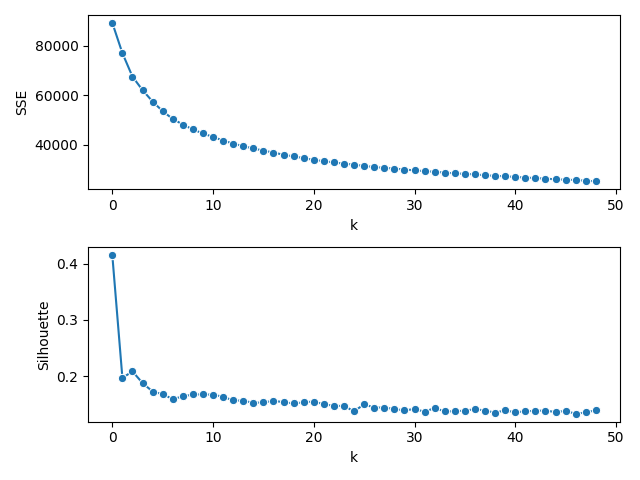
\includegraphics[width=\textwidth]{plots/sse_silh_kmeans.png}
        \caption{SSE and Silhouette scores}
        \label{fig:sse_silh_kmeans}
    \end{subfigure}
    \hfill
    \begin{subfigure}[b]{0.3\textwidth}
        \centering
        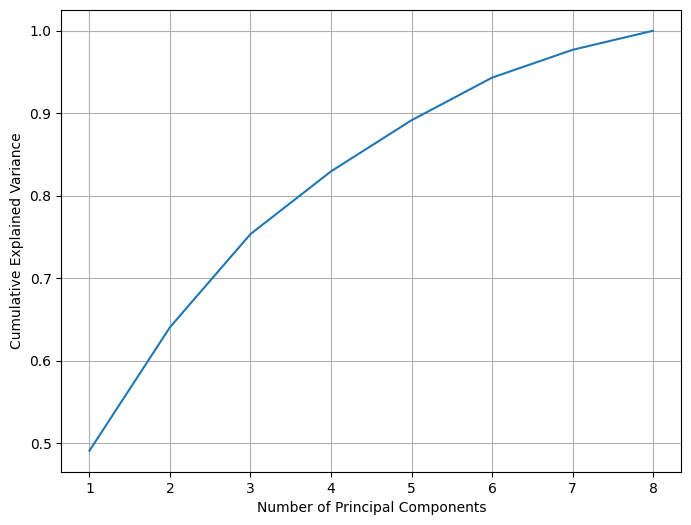
\includegraphics[width=\textwidth]{plots/pca_kmeans.png}
        \caption{PCA Analysis}
        \label{fig:pca_kmeans}
    \end{subfigure}
    \hfill
    \begin{subfigure}[b]{0.3\textwidth}
        \centering
        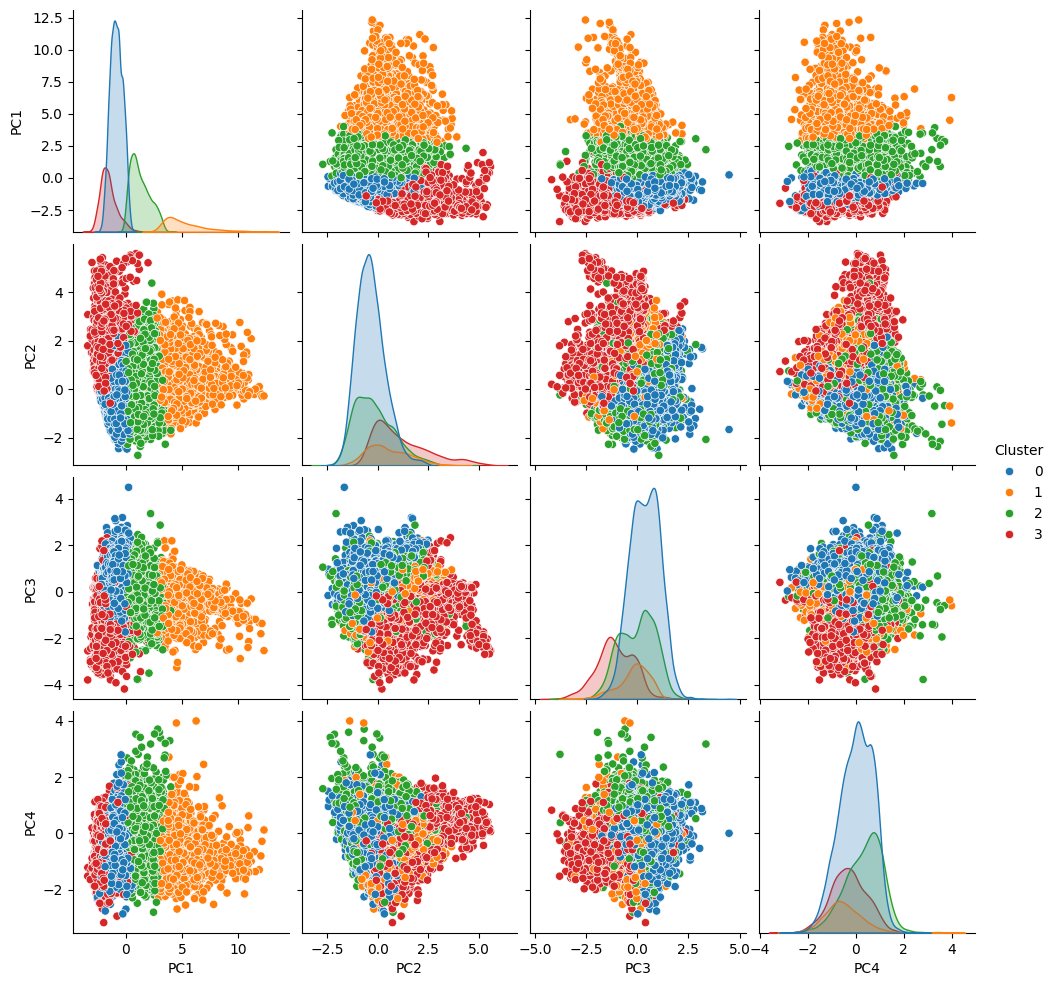
\includegraphics[width=\textwidth]{plots/pairplot_kmeans.png}
        \caption{K-means Visualization}
        \label{fig:pairplot_kmeans}
    \end{subfigure}
    \caption{K-means clustering analysis}
    \label{fig:three_subplots}
\end{figure}
The distribution of data points across the four clusters is as follows (shown in percentages of data points per cluster):
Red (0): 51.68\%, Blue (1): 7.42\%, Green (2): 24.22\%, Orange (3): 16.68\%.
The clusters are not as well-separated in most Principal Component combinations as they are with PC1. 
In fact, in the other combinations, the clusters tend to overlap and their boundaries are not always clearly distinct.
This might be an indication that the true clusters have irregular shapes or different densities, resulting in boundaries between them being not clearly defined.



\section{Density-based methods}\label{sec:density_based}


\section{Analysis by hierarchical clustering}\label{sec:hierarchical}


\section{General considerations}\label{sec:considerations}